\documentclass{ctexart}

\usepackage[dvipsnames]{xcolor}
\usepackage{pgfornamenthan}
\usetikzlibrary{positioning}
\usetikzlibrary{decorations.text}
\usepackage{cncolours}

\usepackage{fullpage}
\usepackage{listings}
\lstset{basicstyle=\ttfamily,columns=fullflexible}

\title{汉风图纹 pgfornament-han}
\author{林莲枝、张辰南}

\begin{document}

\maketitle

\begin{abstract}
利用 pgfornament 宏包可以在 \LaTeX{} 文件里便捷地画出十分典雅漂亮的、英伦风满满的维克多利亚风格花纹。 pgfornament-han 宏包的用意,正是为了尝试用 pgfornament 的已有机制,提供一些汉风的传统图纹。所有图纹均由张辰南以 CAD 程式设计、以 TikZ 画图,再由林莲枝转为适合 pgfornament 机制使用的宏包代码。
\end{abstract}

\emph{(这不是正式帮助文档,只是暂时性的测试文档,内容极大可能会变动。)}

先来一个 \pgfornamenthan[color=blue,scale=0.2]{56} 寿字纹。\pgfornament[scale=0.3]{56} 依然可用。
%
%
玩点花样:
%
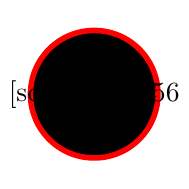
\begin{tikzpicture}
  \tikzset{pgfornamentstyle/.style={draw=Goldenrod,fill=Red,line width=1pt}}
  \node[fill=black,circle,draw=Red,line width=2pt,inner sep=-8pt] at (0,0){%
  \pgfornamenthan[scale=0.38]{56}
};
\end{tikzpicture}

\begin{tikzpicture}[x=1pt,y=1pt]
    \tikzset{every node/.append style={inner sep=0pt,color=胭脂}}
    % \tikzset{pgfornamentstyle/.append style={draw=Goldenrod,fill=Red,line width=1pt}}
      \node (nw) {\pgfornamenthan[scale=0.35]{1}};
    \node[anchor=north west,right=100 of nw] (ne) {\pgfornamenthan[symmetry=v,scale=0.35]{1}};
    \node[anchor=north west,below=0pt of nw] (sw) {\pgfornamenthan[symmetry=h,scale=0.35]{1}};
    \node[anchor=north east,below=0pt of ne] (se) {\pgfornamenthan[symmetry=c,scale=0.35]{1}};

    %% 用 pgfornmanet 自带的 \draw (A) to[ornamenthan=19] (B) 机制的话会导致线条高度跟着变化!只好折衷用tikz的 xscale 来实现加长了。\pgfornamenthan 本身的 scale 则要确保和角点的 scale 一致。
    \node[anchor=north west,xscale=1.45] at (nw.north east) {\pgfornamenthan[scale=0.35]{29}};
    \node[anchor=south west,xscale=1.45] at (sw.south east) {\pgfornamenthan[scale=0.35]{29}};

  \node[font=\kaishu,align=center,xshift=50,text=black] at (nw.south east)
     {给我一片海棠红啊海棠红\\血一样的海棠红\\
     沸血的烧痛是乡愁的烧痛\\给我一片海棠红啊海棠红};
\end{tikzpicture}
%
\hfill
%
\begin{tikzpicture}
  \tikzset{every node/.append style={铜绿,inner sep=0pt}}
  \node (nw) {\pgfornamenthan[scale=0.25]{12}};
  \node[right=50bp of nw] (ne) {\pgfornamenthan[scale=0.25,symmetry=v]{12}};
  \node[below=50bp of nw] (sw) {\pgfornamenthan[scale=0.25,symmetry=h]{12}};
  \node[below=50bp of ne] (se) {\pgfornamenthan[scale=0.25,symmetry=c]{12}};

  % 每个部件原宽度为200bp,因此绘画时如果以bp作为单位,会比较容易计算xscale的值。
  % 这里 scale=0.25 则部件有效宽度为50bp,刚好是两个角点符号之间的距离(参照
  % 上面4行代码),因此不需要再设 xscale。
  \node[anchor=north west] at (nw.north east) {\pgfornamenthan[scale=0.25]{32}};
  \node[anchor=south west] at (sw.south east) {\pgfornamenthan[scale=0.25]{32}};
  \node[anchor=south west,rotate=-90] at (nw.south west) {\pgfornamenthan[scale=0.25]{32}};
  \node[anchor=south east,rotate=90] at (ne.south east) {\pgfornamenthan[scale=0.25]{32}};

  \node[anchor=center,靛蓝,shift={(25bp,-25bp)}] at (nw.south east) {\pgfornamenthan[scale=0.5]{56}};
\end{tikzpicture}



\begin{lstlisting}
\pgfornament[color=red,width=1.5cm]{n}
\end{lstlisting}

TikZ 选项的应用:
\begin{lstlisting}
\tikzset{pgfornamentstyle/.append style={draw=black,fill=red,line width=1}}
\pgfornament[scale=2]{n}
\end{lstlisting}

\noindent%
\foreach \n in {1,...,32,56}{%
  \begin{tikzpicture}
    \fill[牙色](-1cm,-1cm) rectangle (1cm,1cm);
    \node[inner sep=0pt] (element) {\pgfornamenthan[color=茜色,width=1.8cm]{\n}};
    \node[inner sep=0pt,font=\footnotesize] at (0.8cm,-0.8cm) {\n};
  \end{tikzpicture}\space
}

\end{document}
% \bigskip

\noindent%
\foreach \n in {1,...,32,56}{%
% \tikzset{every node/.append style={inner sep=0pt,line width=1}}%
\tikzset{pgfornamentstyle/.append style={draw=藏蓝,fill=枣红,line width=1}}%
\pgfornamenthan[width=2cm]{\n}%
\tikzset{pgfornamentstyle/.append style={line width=1}}%
\pgfornamenthan[width=2cm,symmetry=v,color=水色]{\n}
}

\end{document}
